\documentclass[12pt,a4paper]{scrartcl}
\usepackage[utf8]{inputenc}
\usepackage[english,russian]{babel}
\usepackage{indentfirst}
\usepackage{misccorr}
\usepackage{graphicx}
\usepackage{amsmath}
\usepackage{multirow}
\usepackage{pgfplots}
\usepackage{parskip}
\usepackage[top=1cm, bottom=1cm, left=1cm, right=1cm]{geometry}
\pgfplotsset{compat=1.9}

\begin{document}
	\graphicspath{{/home/cd7567/Pictures/TeXImgs}}
	
	\newcommand{\ms}{\mathstrut}
	\newcommand{\msp}{\hspace{0.5cm}}
	\newcommand{\al}{\alpha}
	\newcommand{\dg}{^\circ}
	\newcommand{\dif}{\mathrm{d}}
	\newcommand{\qd}[2]{^{\frac{#1}{#2}}}
	\newcommand{\qdm}[2]{^{-\frac{#1}{#2}}}
	\newcommand{\lm}[2]{\underset{#1 \rightarrow #2}{\lim}}
	\newcommand{\sfrac}[2]{\dfrac{\strut #1}{\strut #2}}
	\newcommand{\equal}[1]{\overset{(#1)}{=}}
	\newcommand{\linevdots}{\ \raisebox{-.08\height}{\vdots}\ }
	\newcommand{\linecvdots}{\ \raisebox{-.08\height}{\vdots}\hspace{-0.13cm}\raisebox{.15\height}{\cancel{\phantom{a}}\hspace{0.06cm}}}
	\newcommand{\combox}[1]{\ms \msp \msp \begin{minipage}{0.95\linewidth}
			#1
	\end{minipage}}
	
	\newtheorem{pr}{Задача}
	\newtheorem{ex}{Пример}
	\newtheorem{dfn}{Def}
	\newtheorem{theorem}{Th}
	
	\newenvironment{slv}{\ms \msp \textit{Решение:}}{}
	\newenvironment{proof}{\ms \msp \textit{Доказательство: }}{\hfill $\square$}
	
	\begin{titlepage}
		
		\vspace*{\fill}
		
		\begin{center}
			
\includegraphics[scale=0.8]{MIPT.png}
			\\[0.7cm]\Huge Московский Физико-Технический Институт\\(национальный исследовательский университет)
			\\[2cm]\LARGE Отчет по эксперименту
			\\[0.5cm]\noindent\rule{\textwidth}{1pt}
			\\\Huge\textbf{Измерение теплопроводности воздуха\\при атмосферном давлении}
			\\[-0.5cm]\noindent\rule{\textwidth}{1pt}
		\end{center}
		
		\begin{flushleft}
			\textit{Работа №2.2.3; дата: 25.03.22}\hfill\textit{Семестр: 2}
		\end{flushleft}
		
		\vspace*{\fill}
		
		\begin{flushleft}
			Выполнил: \hspace{\fill} Группа:
			\\Кошелев Александр \hspace{\fill} Б05-105
		\end{flushleft}
	\end{titlepage}
	
	%Страница 2
	
	\begin{flushleft}
		\footnotesize{Измерение теплопроводности воздуха при атмосферном давлении} \hspace{\fill} \footnotesize{2}
		\\[-0.3cm]\noindent\rule{\textwidth}{0.3pt}
	\end{flushleft}
	
	\section{Аннотация}
	
	\textbf{Цель работы: }
	
	Измерить коэффициент теплопроводности воздуха при атмосферном давлении в зависимости от температуры.
	
	\textbf{Схема установки:}
	\begin{center}
		\begin{figure}[h]
			\begin{minipage}{0.43\linewidth}
				\begin{center}
					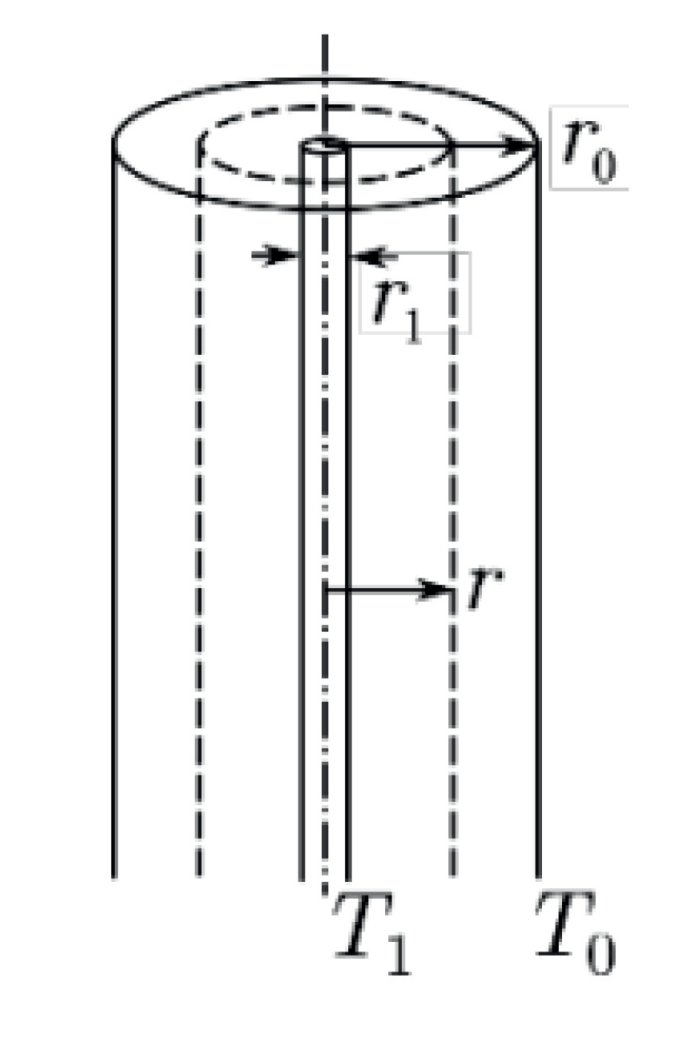
\includegraphics[scale=0.127]{PIC_1.png}
					\\\textbf{Рис. 1:} Cхема установки
				\end{center}
			\end{minipage}
			\begin{minipage}{0.57\linewidth}
				\begin{center}
					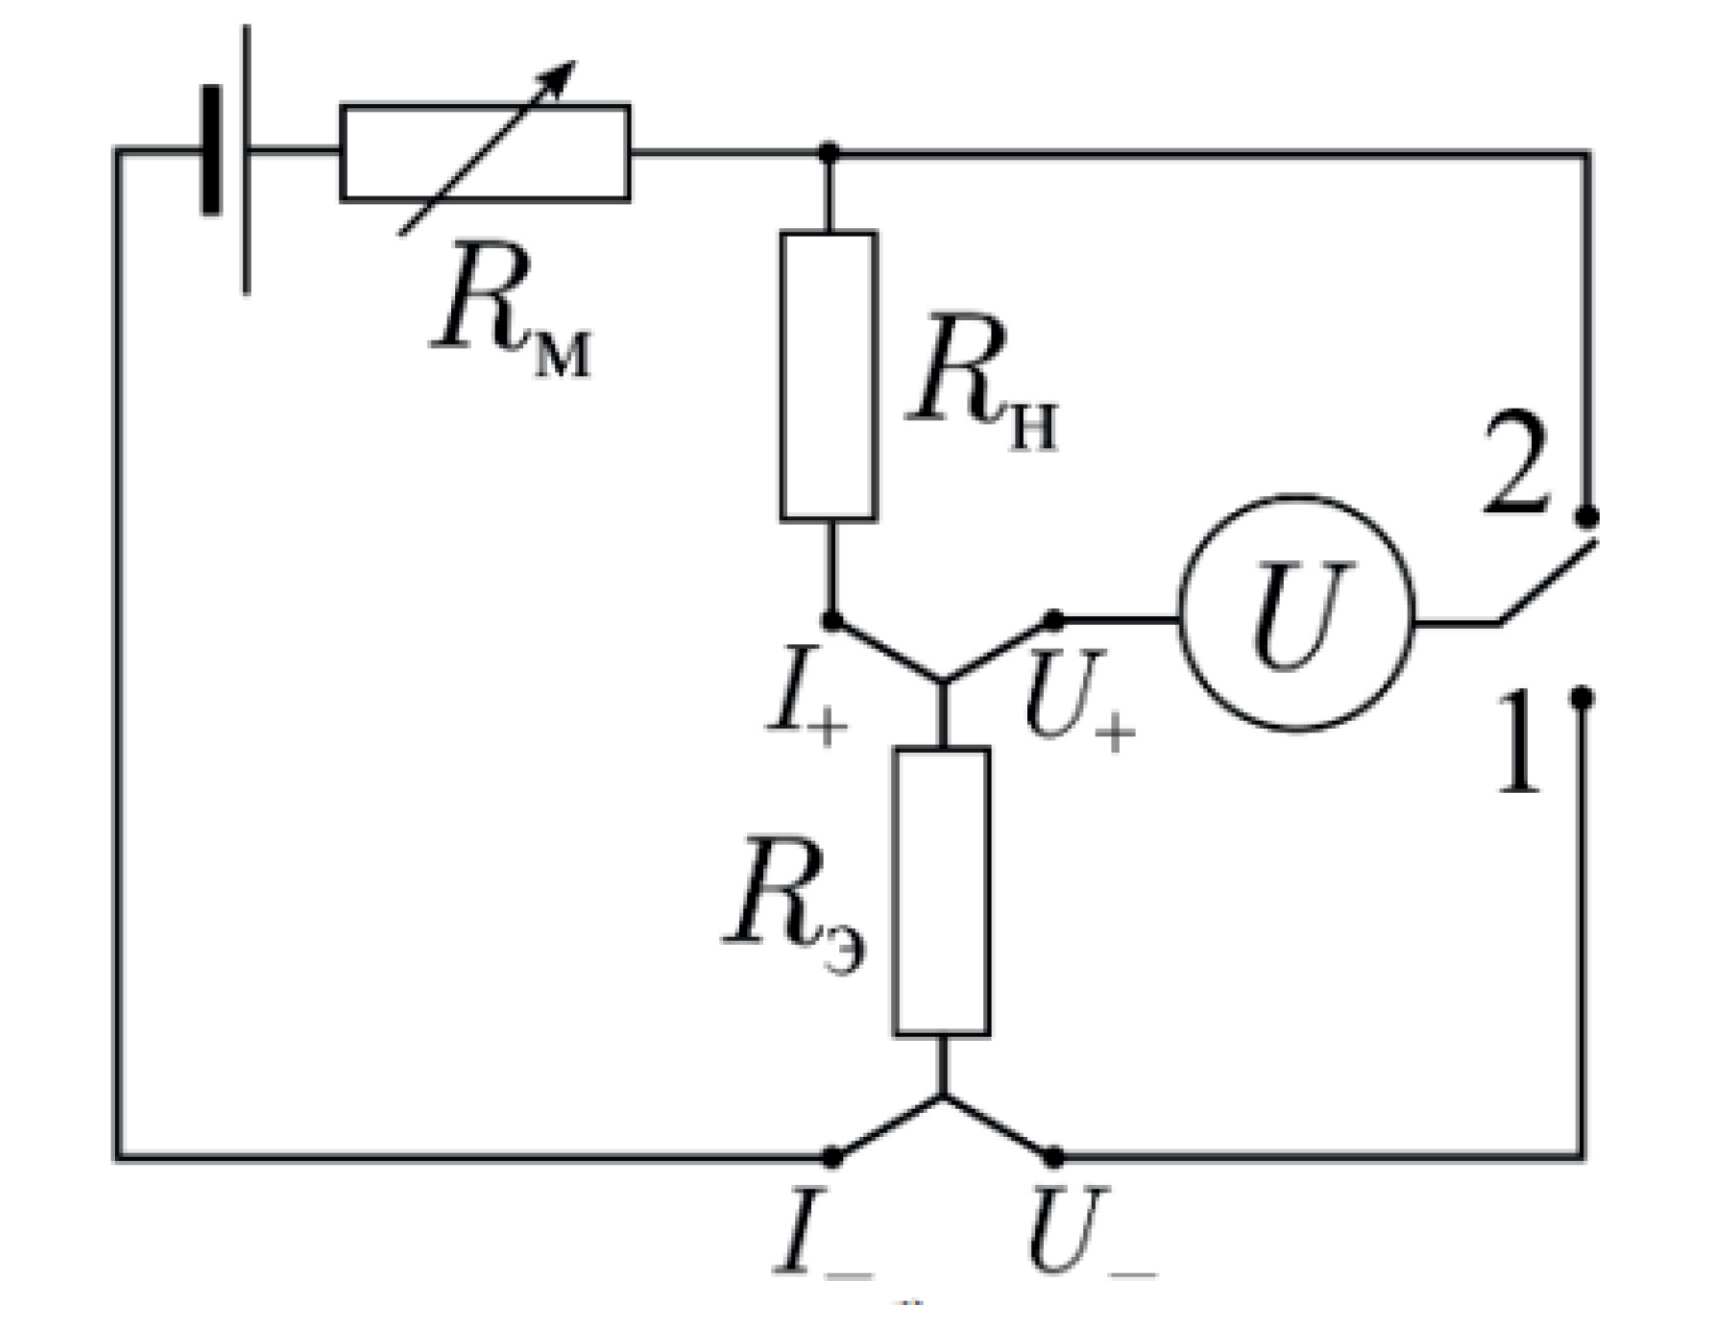
\includegraphics[scale=0.1]{PIC_2.png}
					\\\textbf{Рис. 2:} Электрическая схема установки
				\end{center}
			\end{minipage}
		\end{figure}
	\end{center}
		
	\textbf{В работе используются:}
	
	Цилиндрическая колба с натянутой по оси нитью, термостат, вольтметр и амперметр (цифровые мультиметры), эталонное сопротивление, источник постоянного напряжения, реостат (или магазин сопротивлений).
	
	\section{Теоретические сведения}
	Тепловой поток через воздух в цилиндрическом сосуде можно рассчитать по формуле:
	$$q = \sfrac{2\pi L}{\ln (\frac{r_0}{r_1})}\kappa \Delta T = \sfrac{1}{\beta}\kappa \Delta T$$
	
	Теперь продифференцируем это выражение:
	$$\kappa = \beta \sfrac{\dif q}{\dif (\Delta T)}$$
	
	Таким образом, если построить график зависимости теплового потока от нити от температуры окружающей среды, то коэффициент наклона графика будет пропорционален коэффициенту теплопроводности $k$.
	
	Используя схему 2 теплоту, производимую на нити можно определить по закону Джоуля-Ленца:
	$$q = IU$$
	
	Сопротивление же нити получим по закону Ома:
	$$R = \sfrac{U}{I}$$
	
	Также отметим, что сопротивление нити меняется по температурному закону:
	$$R = R_0(1 + \alpha t)$$
	\newpage 
	
	%Страница 3
	
	\begin{flushleft}
		\footnotesize{Измерение теплопроводности воздуха при атмосферном давлении} \hspace{\fill} \footnotesize{3}
		\\[-0.3cm]\noindent\rule{\textwidth}{0.3pt}
	\end{flushleft}

	\section{Проведение эксперимента}
	\paragraph{Основные параметры при проведении эксперимента} \hfill
	
	Основными параметрами в данной ряботе являются эталонное сопротивление $R_{\text{э}} = 10\, \text{Ом}$, логарифм отношения радиусов цилиндра $\ln \frac{r_0}{r_1} = 5.30$ и длина нити $L = 365\, \text{мм}$.
	\hspace{-1cm}
	\paragraph{Проверка линейности зависимости сопротивления от температуры} \hfill
	\begin{center}
		\begin{tabular}{|c|c|c|c|}
			\hline
			\multicolumn{4}{|c|}{$t = 21.4\,^\circ$C}
			\\\hline
			$U_0$, мВ & $U_{\text{н}}$, мВ & $R_{\text{н}}$, Ом & $q$, мВт
			\\\hline
			$107.8 \pm 0.1$ & $107.4 \pm 0.1$ & $9.96 \pm 0.01$ & $1.16 \pm 0.01$
			\\\hline
			$208.8 \pm 0.1$ & $208.2 \pm 0.1$ & $9.97 \pm 0.01$ & $4.35 \pm 0.01$
			\\\hline
			$555.8 \pm 0.1$ & $558.8 \pm 0.1$ & $10.05 \pm 0.01$ & $31.05 \pm 0.03$
			\\\hline 
			$739.8 \pm 0.1$ & $749.3 \pm 0.1$ & $10.13 \pm 0.01$ & $55.43 \pm 0.06$
			\\\hline
			$1104.0 \pm 0.1$ & $1141.3 \pm 0.1$ & $10.34 \pm 0.01$ & $126.00 \pm 0.13$
			\\\hline
			$1269.0 \pm 0.1$ & $1327.8 \pm 0.1$ & $10.46 \pm 0.01$ & $168.50 \pm 0.17$
			\\\hline
			\multicolumn{4}{|c|}{$t = 30.1\,^\circ$C}
			\\\hline
			$U_0$, мВ & $U_{\text{н}}$, мВ & $R_{\text{н}}$, Ом & $q$, мВт
			\\\hline
			$107.7 \pm 0.1$ & $110.7 \pm 0.1$ & $10.28 \pm 0.01$ & $1.19 \pm 0.01$
			\\\hline
			$208.5 \pm 0.1$ & $214.5 \pm 0.1$ & $10.29 \pm 0.01$ & $4.47 \pm 0.01$
			\\\hline
			$553.7 \pm 0.1$ & $574.2 \pm 0.1$ & $10.37 \pm 0.01$ & $31.79 \pm 0.03$
			\\\hline
			$736.2 \pm 0.1$ & $768.8 \pm 0.1$ & $10.44 \pm 0.01$ & $56.60 \pm 0.06$
			\\\hline
			$1095.5 \pm 0.1$ & $1166.6 \pm 0.1$ & $10.65 \pm 0.01$ & $127.80 \pm 0.13$
			\\\hline
			$1250.8 \pm 0.1$ & $1355.0 \pm 0.1$ & $10.83 \pm 0.01$ & $169.48 \pm 0.17$
			\\\hline
			\multicolumn{4}{|c|}{$t = 40.0\,^\circ$C}
			\\\hline
			$U_0$, мВ & $U_{\text{н}}$, мВ & $R_{\text{н}}$, Ом & $q$, мВт
			\\\hline
			$128.3 \pm 0.1$ & $136.6 \pm 0.1$ & $10.65 \pm 0.01$ & $1.75 \pm 0.01$
			\\\hline
			$208.3 \pm 0.1$ & $221.9 \pm 0.1$ & $10.65 \pm 0.01$ & $4.62 \pm 0.01$
			\\\hline
			$552.3 \pm 0.1$ & $593.0 \pm 0.1$ & $10.74 \pm 0.01$ & $32.75 \pm 0.04$
			\\\hline
			$733.9 \pm 0.1$ & $793.0 \pm 0.1$ & $10.81 \pm 0.01$ & $58.20 \pm 0.06$
			\\\hline
			$1091.0 \pm 0.1$ & $1200.9 \pm 0.1$ & $11.01 \pm 0.01$ & $131.02 \pm 0.13$
			\\\hline
			$1250.8 \pm 0.1$ & $1393.2 \pm 0.1$ & $11.13 \pm 0.01$ & $174.37 \pm 0.18$
			\\\hline
			\multicolumn{4}{|c|}{$t = 50.0\,^\circ$C}
			\\\hline
			$U_0$, мВ & $U_{\text{н}}$, мВ & $R_{\text{н}}$, Ом & $q$, мВт
			\\\hline
			$107.6 \pm 0.1$ & $118.4 \pm 0.1$ & $11.00 \pm 0.01$ & $1.27 \pm 0.01$
			\\\hline
			$208.0 \pm 0.1$ & $229.2 \pm 0.1$ & $11.02 \pm 0.01$ & $4.77 \pm 0.01$
			\\\hline
			$550.9 \pm 0.1$ & $611.4 \pm 0.1$ & $11.10 \pm 0.01$ & $33.68 \pm 0.03$
			\\\hline
			$731.1 \pm 0.1$ & $816.6 \pm 0.1$ & $11.17 \pm 0.01$ & $59.70 \pm 0.06$
			\\\hline
			$1084.5 \pm 0.1$ & $1233.7 \pm 0.1$ & $11.38 \pm 0.01$ & $133.79 \pm 0.12$
			\\\hline
			$1243.5 \pm 0.1$ & $1429.5 \pm 0.1$ & $11.50 \pm 0.01$ & $177.76 \pm 0.16$
			\\\hline
			\multicolumn{4}{|c|}{$t = 60.0\,^\circ$C}
			\\\hline
			$U_0$, мВ & $U_{\text{н}}$, мВ & $R_{\text{н}}$, Ом & $q$, мВт
			\\\hline
			$107.5 \pm 0.1$ & $122.3 \pm 0.1$ & $11.38 \pm 0.01$ & $1.31 \pm 0.01$
			\\\hline
			$207.8 \pm 0.1$ & $236.7 \pm 0.1$ & $11.39 \pm 0.01$ & $4.92 \pm 0.01$
			\\\hline
			$549.2 \pm 0.1$ & $630.0 \pm 0.1$ & $11.47 \pm 0.01$ & $34.60 \pm 0.03$
			\\\hline
			$728.2 \pm 0.1$ & $840.5 \pm 0.1$ & $11.54 \pm 0.01$ & $61.21 \pm 0.05$
			\\\hline
			$1078.3 \pm 0.1$ & $1266.5 \pm 0.1$ & $11.75 \pm 0.01$ & $136.57 \pm 0.12$
			\\\hline
			$1258.2 \pm 0.1$ & $1495.1 \pm 0.1$ & $11.88 \pm 0.01$ & $188.11 \pm 0.16$
			\\\hline
		\end{tabular}
		\\\textbf{Табл. 2:} Рассчет сопротивления и мощности
	\end{center}

	\newpage
	
	%Страница 4
	
	\begin{flushleft}
		\footnotesize{Измерение теплопроводности воздуха при атмосферном давлении} \hspace{\fill} \footnotesize{4}
		\\[-0.3cm]\noindent\rule{\textwidth}{0.3pt}
	\end{flushleft}
	
	Из построения по предыдущей таблице получаем нагрузочные кривые $R(Q)$ для разных температур. Сами графики приводить не будем, оформим в таблицу полученные аппроксимацией значения $R(0)$, соответствующие сопротивлению при данных температурах.
	
	\begin{center}
		\begin{tabular}{|c|c|c|c|c|c|}
			\hline
			$t$, $^\circ$C & $21.4 \pm 0.1$ & $30.1 \pm 0.1$ & $40.0 \pm 0.1$ & $50.0 \pm 0.1$ & $60.0 \pm 0.1$
			\\\hline
			$R$, Ом & $9.958 \pm 0.005$ & $10.270 \pm 0.005$ & $10.644 \pm 0.005$ & $11.003 \pm 0.005$ & $11.377 \pm 0.004$
			\\\hline
		\end{tabular}
		\\\textbf{Табл. 3:} Зависимость $R(t)$
	\end{center}
	
	Построим график зависимости $R(t)$ для проверки теоретической зависимости.
	
	\begin{center}
		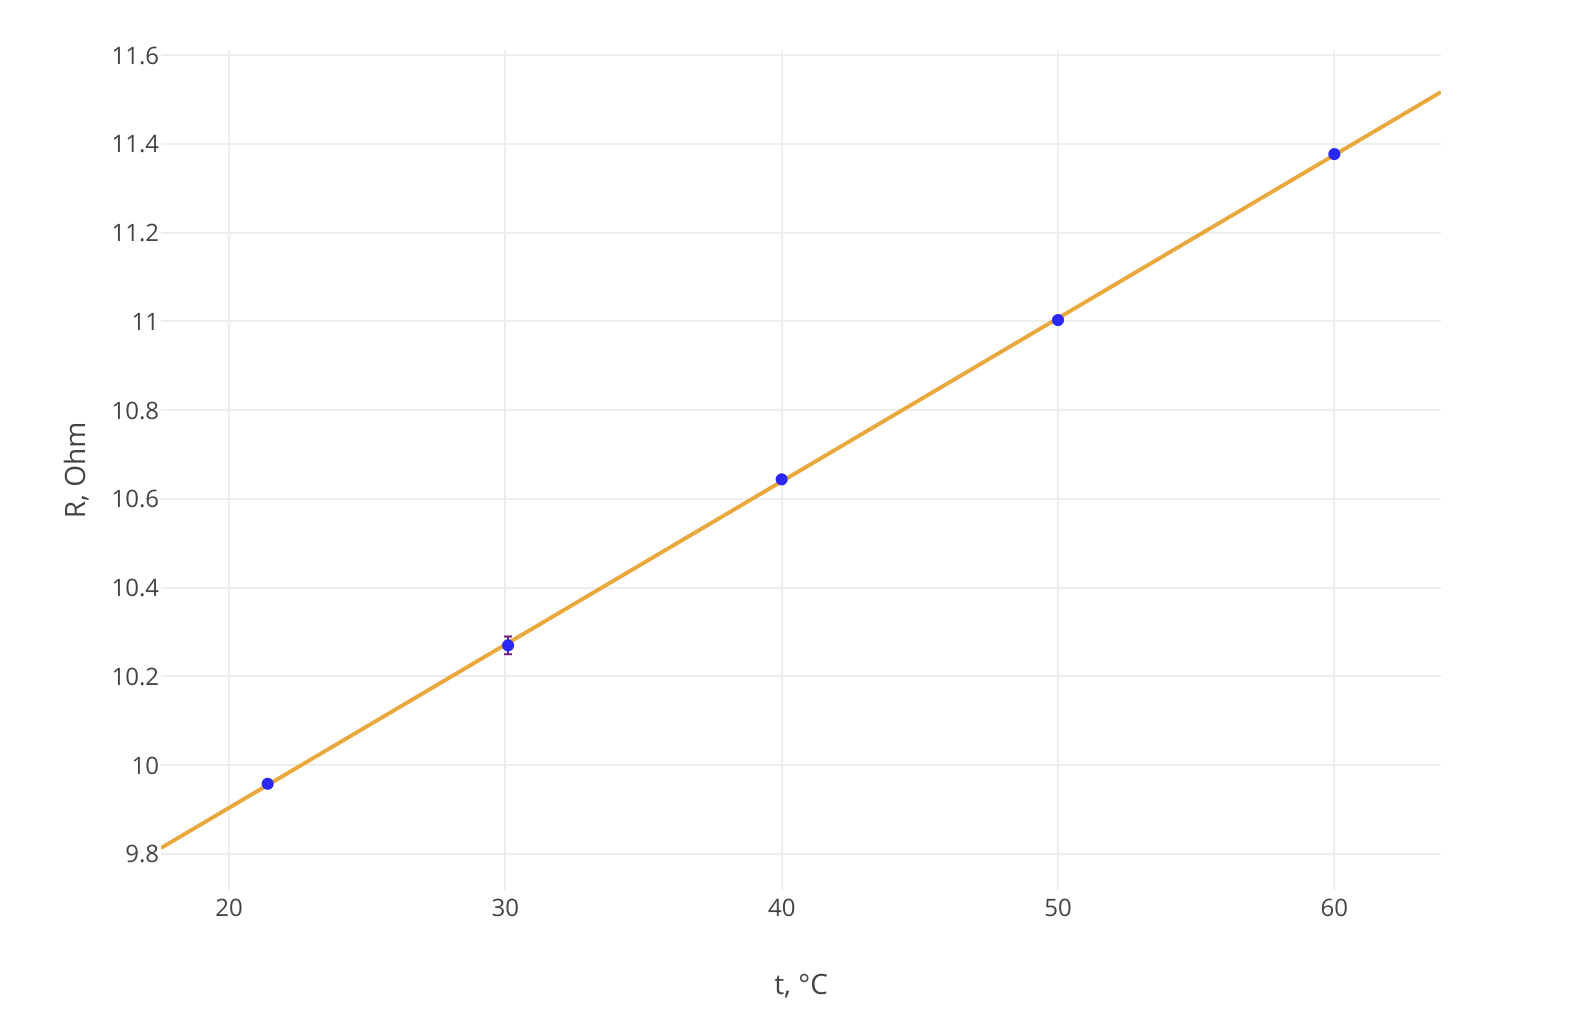
\includegraphics[scale=0.25]{PIC_3.png}
		\\\textbf{Рис. 3:} График зависимости $R(t)$
	\end{center}
	
	В самом деле, зависимость получается линейной, как и предполагается теоретически. Можем подсчитать $R_0$ -- сопротивление при реперной температуре и $\alpha$ -- коэффициент наклона.
	
	$$R_0 = (9.168 \pm 0.014)\,\text{Ом}$$
	$$\alpha = (0.0368 \pm 0.0003)\,\text{Ом}/^\circ \text{C}$$
	
	\paragraph{Определение коэффициента теплопроводности} \hfill
	
	По графикам для конкретных температур из предыдущего пункта в таблице выпишем соответствующие значения $\kappa$ и построим график зависимости $\kappa(T)$ в линейных и двойных логарифмических координатах.
	
	\begin{center}
		\begin{tabular}{|c|c|c|c|c|c|}
			\hline
			$T$, К & $294.5 \pm 0.1$ & $303.2 \pm 0.1$ & $313.1 \pm 0.1$ & $323.1 \pm 0.1$ & $333.1 \pm 0.1$
			\\\hline
			$\ln T/T_0$ & $0.0758 \pm 0.0003$ & $0.1049 \pm 0.0003$ & $0.1371 \pm 0.0003$ & $0.1685 \pm 0.0003$ & $0.1990 \pm 0.0003$
			\\\hline
			$\frac{\dif R}{\dif Q}$, Ом/мДж & $0.0030 \pm 0.0001$ & $0.0032 \pm 0.0002$ & $0.0031 \pm 0.0002$ & $0.0028 \pm 0.0001$ & $0.0027 \pm 0.0001$
			\\\hline
			$\frac{\dif R}{\dif T}$, Ом/К & \multicolumn{5}{|c|}{$0.0368 \pm 0.0003$}
			\\\hline
			$\kappa$, Вт/м$\,\cdot\,$К & $0.027 \pm 0.001$ & $0.028 \pm 0.002$ & $0.028 \pm 0.002$ & $0.031 \pm 0.001$ & $0.032 \pm 0.001$
			\\\hline
			$\ln \kappa/\kappa_0$ & $0.093 \pm 0.011$ & $0.130 \pm 0.012$ & - & $0.231 \pm 0.012$ & $0.263 \pm 0.013$
			\\\hline 
		\end{tabular}
		\\\textbf{Табл. 4:} Таблица зависимости $\kappa(T)$
	\end{center}
	
	\newpage
	
	%Страница 5
	
	\begin{flushleft}
		\footnotesize{Измерение теплопроводности воздуха при атмосферном давлении} \hspace{\fill} \footnotesize{5}
		\\[-0.3cm]\noindent\rule{\textwidth}{0.3pt}
	\end{flushleft}
	
	\begin{center}
		\begin{figure}[h]
			\begin{minipage}{0.5\linewidth}
				\begin{center}
					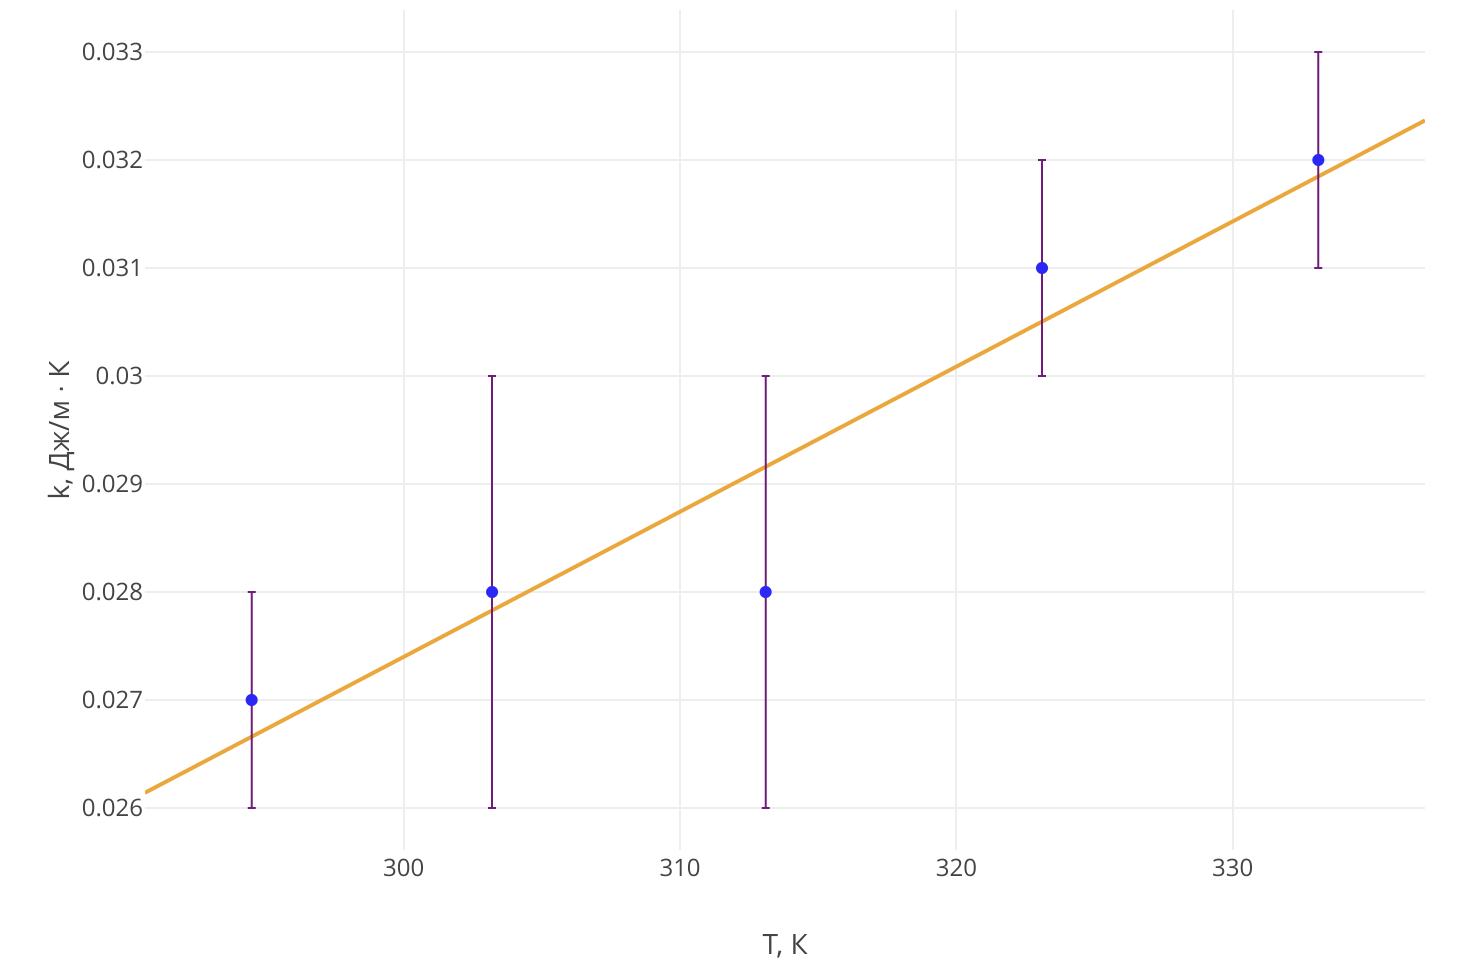
\includegraphics[scale=0.15]{PIC_4}
					\\\textbf{Рис. 4:} Зависимость $\kappa(T)$
				\end{center}
			\end{minipage}
			\begin{minipage}{0.5\linewidth}
				\begin{center}
					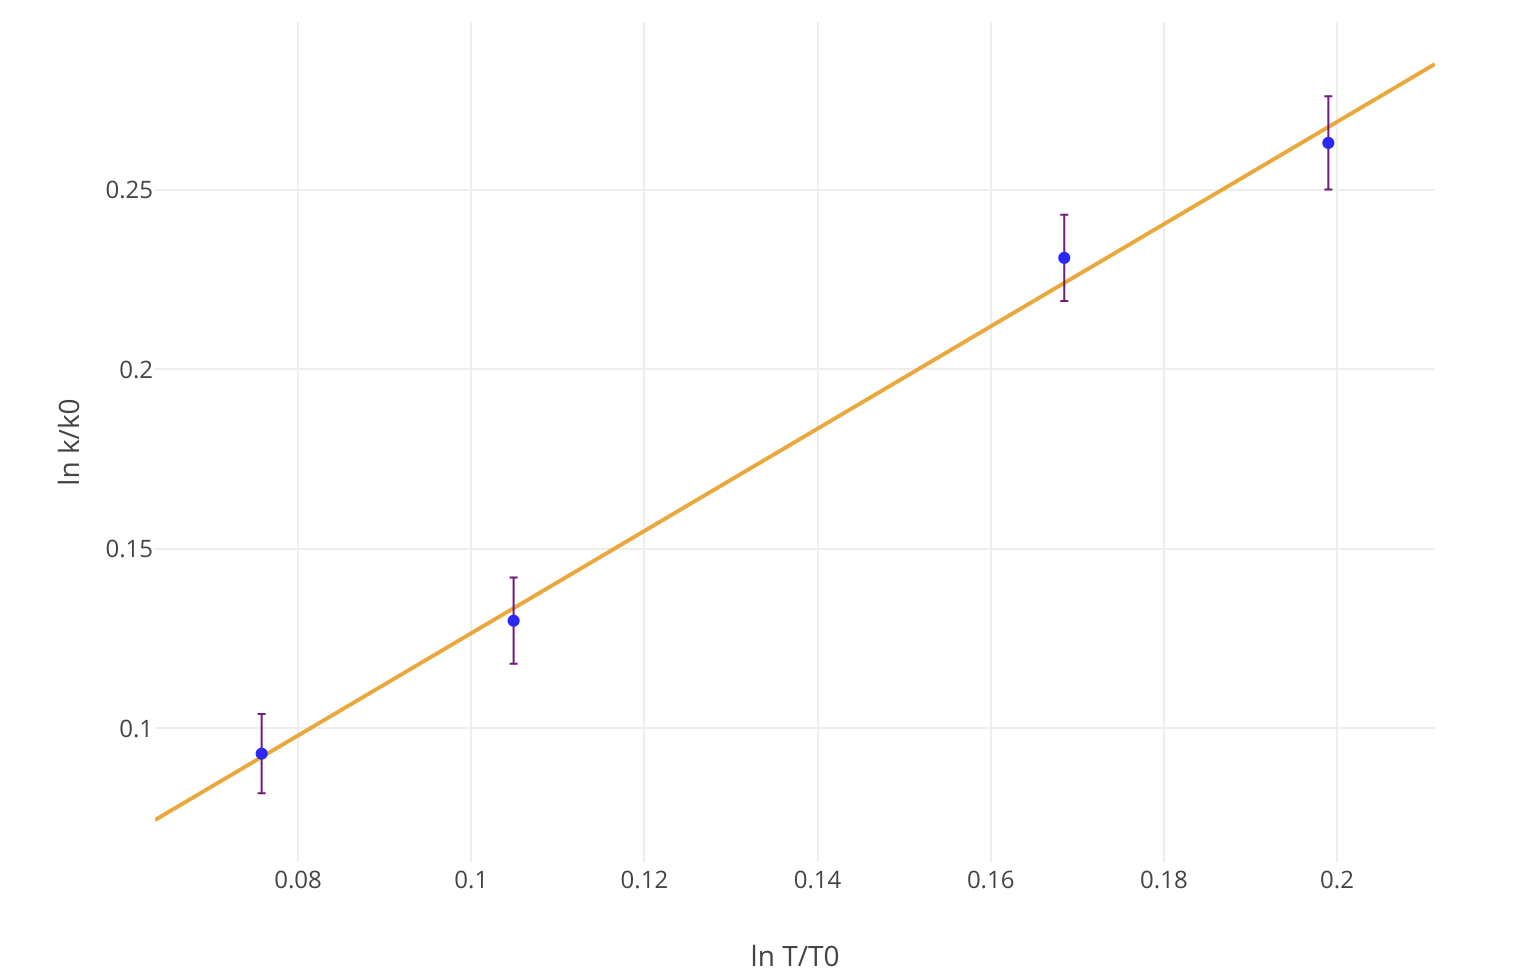
\includegraphics[scale=0.15]{PIC_5}
					\\\textbf{Рис. 5:} Зависимость $\ln \kappa/\kappa_0(\ln T/T_0)$
				\end{center}
			\end{minipage}
		\end{figure}
	\end{center}
	
	Если считать заранее известным вид зависимости. можно экстраполировать график Рис. 4 и получить значение $\kappa_0$ соответствующее $0^\circ$C. Явно заметна точка, значение которой -- случайный выброс. Ее уберем из рассмотрения. Таким образом, из этих графиков получаем зависимость
	$$\kappa \sim T^{\lambda},\ \ \lambda = (1.42 \pm 0.13)$$
	
	
	\section{Выводы}
	\begin{enumerate}
		\item В результате работы получены и представлены в таблице 4 значения теплопроводности воздуха.
		\item В предположении $\kappa \sim T^\lambda$ получено значение $\lambda = \lambda = (1.42 \pm 0.13)$. Этот результат не согласуется с теорией, т.к теоретически зависимость вида $\kappa \sim \sqrt{T}$. Объяснить такую ошибку можно случайными ошибками при проведении эксперимента, или неучтенными систематическими эффектами, влияющими на результат.
	\end{enumerate}
	
\end{document}